\documentclass[conference]{IEEEtran}
\usepackage[T1]{fontenc}
\renewcommand{\ttdefault}{lmtt}
\usepackage{amsmath,amssymb,booktabs,graphicx,microtype,xcolor,url}
\usepackage{tikz}
\usetikzlibrary{arrows.meta,positioning}
\usepackage[hidelinks]{hyperref}
\hypersetup{pdftitle={Bad Blood V2 - Final Results 20261015},pdfauthor={Jingyi Guo}}
\pagestyle{plain}
\setlength{\emergencystretch}{1.5em}
\newcommand{\pair}{\textsc{PairSE}}
\newcommand{\pkg}{\texttt{final\_results\_20261015}}
\title{Bad Blood V2: Attention-Based Population Models\protect\\and Reference-Conditioned Personalization}
\author{\IEEEauthorblockN{Jingyi Guo}
\IEEEauthorblockA{Bad Blood Project, University of Notre Dame\\
Research and Engineering Results Report --- October 15, 2026}}

\begin{document}\maketitle\thispagestyle{plain}
\begin{abstract}
Bad Blood V2 combines a compact population convolutional neural network with
Squeeze-and-Excitation (CNN+SE) and reference-conditioned PairSE personalization.
This 20261015 release adopts personal tail adaptation: the change head, last
residual CNN block and its SE gate are fitted separately for each participant.
Both photoplethysmogram-only (PPG) and electrocardiogram-plus-PPG (ECG+PPG)
versions are retained. Each person's first 80\% of ordered segments supplies
training and three temporal validation periods; their last 20\% is test.
Learning rate and update count are selected independently for systolic and
diastolic blood pressure (SBP/DBP). Across 30 participants and three source seeds,
participant-macro mean absolute error (MAE) is 6.89/4.29 mmHg for PPG and
7.14/4.31 for dual input. Relative to matched additive bias correction, these
are reductions of 19.0/20.3\% and 21.5/24.4\%. Both endpoints improve in the
overall mean in every seed. We retain complete controls, individual outcomes,
checkpoints and runnable code; the previously examined cohort makes this an
exploratory comparison rather than independent external confirmation.
\end{abstract}
\begin{IEEEkeywords}blood pressure, personalization, temporal validation,
PPG, ECG, CNN, Squeeze-and-Excitation\end{IEEEkeywords}

\section{Adopted method and scope}
The adopted personal method is \textbf{tail adaptation with person-specific,
endpoint-specific hyperparameters}. Single and dual signals are two input
versions of this one method. Head-only fitting and automatic selection between
head and tail were evaluated as controls, not retained as alternative deployment
policies. The population model and its source training remain unchanged.
The reported tail policy includes a validation-selected source checkpoint with
zero extra personal updates. This candidate is retained exactly as evaluated;
the fitting rules and recorded test outcomes are unchanged in this release.

\section{Data and matching}
All results use the VitalDB-derived portion of PulseDB \cite{wang2023pulsedb},
not the entire MIMIC-III/VitalDB collection or Notre Dame student recordings.
Source CNN+SE training used 1,085 people / 390,600 ten-second windows, validation
192 / 69,120 and main testing 141 / 56,400. Population main-test MAE remains
12.39/8.00 mmHg for ECG+PPG and 12.32/7.85 for PPG-only. These uncalibrated
population results are a different task and cohort from personal testing.

Personal evaluation randomly selected 30 of 39 eligible local individual records
using seed 20261015, excluding population train/validation/test participants
and the four previous personal-development people. The 30 people and their
indices are identical to the preceding personal-selection experiment.
The first 80\% of chronologically ordered eligible segments provides 8,882
development windows. A ten-second temporal guard precedes the final test period,
which contains 2,211 windows in total. Splits are not random within a person.
Each participant supplies the same development and test data to every control.
These target records have been examined in previous experiments; no final-test
labels entered this run's fitting or selection, but reuse limits confirmatory
interpretation. Earlier six-/sixteen-person, 20\%-support results remain in
the dated 20261013 archive and are not pooled with this new protocol.

Each input is a filtered, synchronized ten-second waveform at 125 Hz (1,250
samples/channel), min-max scaled independently per channel and segment.
ECG then PPG occupy the two input slots; PPG-only zeros the ECG slot throughout
source training, reference encoding and inference. PulseDB's ABP-derived scalar
SBP/DBP labels provide the targets. No current ABP waveform or current true BP
is an inference input. An earlier known scalar BP plus earlier signal is needed
for calibration; intermittent cuff labels are format-compatible but constitute
a separate, much sparser evaluation setting.
\section{Population architecture and training}
\subsection{Signal representation and network}
The supplied filtered ECG and PPG fields are scaled independently within each
window to the unit interval. The tensor shape is $N\times2\times1250$, ordered
ECG then PPG. The PPG-only fit is trained from scratch without ECG. An internal
mask zeros ECG in both ordinary forward inference and reference encoding.
Keeping the two-slot representation maintains a controlled parameter-matched
comparison; it is not a claim that ECG is needed for the PPG model.

\begin{table}[t]\centering\small
\caption{CNN+SE architecture; shapes omit batch dimension.}
\label{tab:layers}
\begin{tabular}{lp{2.45in}}\toprule
Stage & Operation and output\\\midrule
Input & 2 channels $\times$ 1,250 samples; no initial decimation\\
Stem & Conv1d 2$\to$8, kernel 7, stride 2, pad 3; BN; SiLU. $8\times625$\\
Block1 & Residual 8$\to$16, stride 2. $16\times313$\\
Block2 & Residual 16$\to$32, stride 2. $32\times157$\\
Block3 & Residual 32$\to$48, stride 2. $48\times79$\\
SE gate & Temporal mean; Linear 48$\to$6; ReLU; Linear 6$\to$48; sigmoid; multiply channels\\
Readout & Global temporal mean; dropout 0.15; Linear 48$\to$32; SiLU; Linear 32$\to$2\\\bottomrule
\end{tabular}\end{table}

Each residual block has a kernel 7 convolution, BN and SiLU, followed by a
kernel 5 convolution and BN. A stride-matched kernel 1 projection and BN form
the skip branch; SiLU follows the sum. The SE mechanism \cite{hu2018se}
reweights learned feature channels after the final residual stage. These
channels mix signal features; their weights are not direct sensor importance
scores. CBAM and temporal-only attention were also compared using the same
backbone. Adding SE increases parameters from 37,666 to 38,296, about 1.7\%.

\subsection{Objective, optimizer and checkpoint selection}
For normalization $N(\cdot)$, the physical-unit population prediction is
\begin{equation}
 p(X)=\mu+\sigma\odot f_\theta(N(X)),
\end{equation}
where training-only label center $\mu=(115.41765,62.92810)$ and scale
$\sigma=(18.94188,12.08322)$ are stored in the checkpoint. The objective is
mean squared error in standardized SBP/DBP, not a mixture of test metrics.
Both modes use AdamW, learning rate 0.001, weight decay 0.001, batch 256, input
noise SD 0.003 and gradient-norm clipping at 5. A plateau scheduler halves the
learning rate after three validation non-improvements. Maximum training is 40
epochs, with early-stopping patience 8. Checkpoints minimize the mean of SBP
and DBP participant-macro validation MAE. All six SE fits stopped after nine
epochs and retained epoch 1 (Table~\ref{tab:epochs}); later epochs were evaluated
but did not improve that criterion. Seeds 42,43,44 quantify training variation.
Seed 42 is the representative within each modality because its validation score
is best, not because of a test-set ranking.

\begin{table}[t]
\centering\caption{Population fits and validation-selected checkpoints. Bold: lowest validation score per input configuration.}\label{tab:epochs}
\scriptsize
\setlength{\tabcolsep}{4pt}
\begin{tabular}{lrrrr}\toprule
Input & Seed & Run epochs & Best epoch & Val. score\\\midrule
dual & 42 & 9 & 1 & \textbf{10.291}\\
dual & 43 & 9 & 1 & 10.457\\
dual & 44 & 9 & 1 & 10.421\\
ppg & 42 & 9 & 1 & \textbf{10.374}\\
ppg & 43 & 9 & 1 & 10.583\\
ppg & 44 & 9 & 1 & 10.406\\
\bottomrule\end{tabular}
\end{table}

\begin{table}[t]
\centering\caption{Dual-input architectures: three-seed participant-macro MAE (SBP / DBP), mmHg. Bold: lowest per pressure and split.}\label{tab:architecture}
\scriptsize
\setlength{\tabcolsep}{4pt}
\begin{tabular}{lrrr}\toprule
Model & Parameters & Validation & Main test\\\midrule
Plain CNN & 37666 & \textbf{12.41} / 8.33 & 12.59 / 8.36\\
CNN+SE & 38296 & 12.51 / \textbf{8.26} & \textbf{12.39} / \textbf{8.00}\\
CNN+temporal & 37680 & 12.49 / 8.32 & 12.58 / 8.31\\
CNN+CBAM & 38310 & 12.52 / 8.29 & 12.42 / 8.11\\
CNN+additive & 38296 & 12.44 / 8.34 & 12.66 / 8.18\\
CNN+SE-all & 38670 & 12.47 / 8.32 & 12.49 / 8.23\\
\bottomrule\end{tabular}
\end{table}



\section{Reference-conditioned architecture}
PairSE shares one CNN+SE encoder between an earlier reference waveform and a
currently observed waveform. Its 48-dimensional features and two standardized
population predictions are denoted $h_r,p_r$ and $h_c,p_c$. With known reference
BP $y_r$, it constructs
\begin{align}
z_{cr}&=[h_c-h_r,h_r,y_r,p_c-p_r],\\
z_{rr}&=[0,h_r,y_r,0],\\
\widehat y_{c\mid r}&=y_r+(p_c-p_r)+g_\phi(z_{cr})-g_\phi(z_{rr}).
\end{align}
The pressure-change multilayer perceptron (MLP) is 100--64--32--2 with Sigmoid
Linear Unit (SiLU) activations and 8,610 parameters. Full PairSE has 46,906
parameters. Identity subtraction recovers the known BP exactly when both inputs
are identical. Final prediction averages over every known reference in that
person's development bank. Features and BP use distinct, source-training-only
normalization statistics. This is current-pressure estimation using observed
current signals, not prediction of an unseen future waveform.

The design adapts paired-reference and transfer-learning ideas
\cite{mekonnen2024,schlesinger2020,leitner2022}, rather than reproducing their
published networks. We combine a compact 1D residual encoder, a final-stage
SE gate, explicit reference BP, identity anchoring and all-reference averaging.
Group pair-head training freezes the encoder and trains on the same 390,600
source windows with random non-self references from the same participant.
It uses Adam, learning rate 0.001, batch 2,048, standardized mean squared error
(MSE), gradient clipping at 5, at most 20 epochs and patience 5. Source validation
selects checkpoints; target-person data is absent from this group training.

\section{Personal tail adaptation: exact pipeline}
\subsection{Trainable and frozen parameters}
The trainable components are \texttt{change.*}, \texttt{encoder.body.6.*} and
\texttt{encoder.gates.6.*}: the change head, last residual block and final SE
gate, totaling \textbf{33,336 parameters}. Earlier encoder blocks, population
readout weights, feature/BP normalization and BatchNorm running statistics
remain fixed. BatchNorm affine scale/bias inside the last block can change.
Dropout is disabled during personal fitting. The frozen population readout
can still produce different values because its input features are adapted.

\begin{figure}[t]\centering
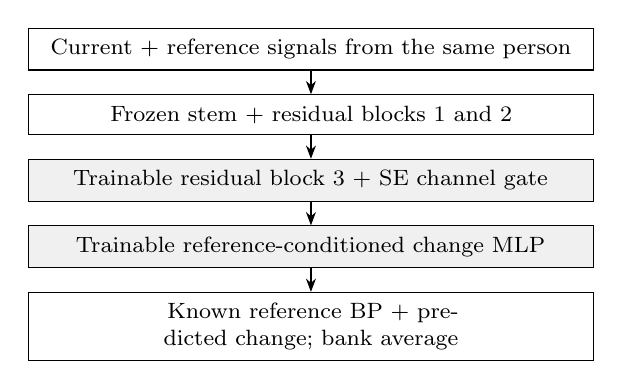
\begin{tikzpicture}[font=\footnotesize,node distance=3mm,
box/.style={draw,align=center,text width=6.9cm,inner sep=4pt},>=Stealth]
\node[box] (a) {Current + reference signals from the same person};
\node[box,below=of a] (b) {Frozen stem + residual blocks 1 and 2};
\node[box,below=of b,fill=black!6] (c) {Trainable residual block 3 + SE channel gate};
\node[box,below=of c,fill=black!6] (d) {Trainable reference-conditioned change MLP};
\node[box,below=of d] (e) {Known reference BP + predicted change; bank average};
\draw[->](a)--(b);\draw[->](b)--(c);\draw[->](c)--(d);\draw[->](d)--(e);
\end{tikzpicture}
\caption{Adopted personal adaptation. Gray components update on one person's
data; early reference and current branches share the same weights.}
\end{figure}

\subsection{Only the person's first 80\% selects their settings}
For each person and source seed, create three expanding temporal folds within
their development bank: train 0--50\%, validate 50--65\%; train 0--65\%, validate
65--80\%; train 0--80\%, validate 80--100\%. These percentages are of the
\emph{development bank}, not the complete recording. Validation starts at least
10 seconds after the latest training window ends. The last 20\% of the full
record is never used in these folds. Candidate fitting always restarts from
the same source PairSE checkpoint.

For each endpoint separately, evaluate learning rates $\{10^{-4},3\times10^{-4}\}$
and update counts $\{10,25,50,100\}$, plus the source model with zero personal
updates. Minimize the equally weighted average of the three validation MAEs.
Ties prefer fewer updates, then smaller learning rate. SBP and DBP may select
different settings; another target person's data has no role in that choice.
After selection, restart from source and refit on the entire development bank.
There are two saved endpoint copies per participant/source seed. Predictions
take SBP from its selected copy and DBP from its selected copy, not both outputs
from an arbitrarily chosen checkpoint.

Every optimizer step uses all valid chronological reference/current pairs in
that fold's training bank, requiring reference end + 10 seconds $\leq$ current
start. The endpoint-specific objective is standardized MSE; the optimizer is
Adam, with no weight decay and gradient norm capped at 5. Update counts are
optimizer steps, not epochs. Pairing reuses observed labels and creates no new
independent observations. Frozen early features are cached; exact accumulated
pair gradients propagate through the trainable tail. Final testing freezes all
weights and uses only known development references and later signal inputs.

\subsection{Controls and source seeds}
Personal mean predicts the mean development BP. Additive bias correction is
$p(X_c)+|S|^{-1}\sum_{r\in S}[y_r-p(X_r)]$, using the same modality's population
model. It already tracks waveform-dependent changes, unlike the constant mean.
Other matched controls are the old fixed head-only PairSE (learning rate
0.0003, 25 joint-endpoint updates), previous single-period personal selection,
three-fold endpoint-specific head-only fitting, and validation-selected head/tail
scope. Only the tail candidate group is the adopted method.

Seeds 42/43/44 change the population training initialization, shuffled training
order and stochastic source pair-head training, yielding different initializers.
They do not change participants, temporal splits or reference budgets.
Personal fitting uses all valid pairs, rather than a newly randomized subset.
Three-seed averages are averages of separate evaluated runs, not an ensemble.

\section{Metrics and overall results}
We compute MAE, root MSE (RMSE), signed Bias, sample error standard deviation
(SD, denominator $n-1$), and fractions within 5, 10 and 15 mmHg, separately for
SBP/DBP. Participant-macro metrics give each of the 30 people equal weight;
pooled metrics give each test segment equal weight. Macro SD averages each
person's error SD and differs from pooled SD. All tables average three seeds.
Best values are bold within each table and endpoint; Bias is ranked by distance
from zero. Full per-person and per-seed metrics are available in the release.

\subsection{PPG only}
Tail adaptation reaches 6.89 / 4.29 mmHg MAE. Relative to personal mean, this is a reduction of 5.35 / 1.73 mmHg (43.70 / 28.77\%). Relative to additive bias correction, the reduction is 1.62 / 1.09 mmHg (19.00 / 20.34\%). Both endpoints improve in the overall mean in each of the three seeds.
\begin{table}[ht]\centering\caption{PPG only: participant-macro results. SBP / DBP.}\scriptsize\setlength{\tabcolsep}{3pt}
\begin{tabular}{lrrr}\toprule
Metric & Personal mean & Bias correction & Tail adaptation\\\midrule
MAE & 12.24 / 6.02 & 8.51 / 5.38 & \textbf{6.89} / \textbf{4.29}\\
RMSE & 14.32 / 7.11 & 10.12 / 6.17 & \textbf{8.51} / \textbf{5.16}\\
Signed Bias & -6.07 / -2.80 & -2.81 / -1.48 & \textbf{-0.70} / \textbf{-0.74}\\
Sample error SD & 9.13 / 4.69 & 7.12 / 3.89 & \textbf{6.52} / \textbf{3.68}\\
$\leq5$ (\%) & 31.14 / 58.60 & 42.98 / 59.35 & \textbf{47.14} / \textbf{65.91}\\
$\leq10$ (\%) & 56.26 / 81.76 & 70.29 / 86.43 & \textbf{75.87} / \textbf{92.65}\\
$\leq15$ (\%) & 72.42 / 89.22 & 85.07 / 94.18 & \textbf{90.50} / \textbf{98.91}\\
\bottomrule\end{tabular}\end{table}

\subsection{ECG+PPG}
Tail adaptation reaches 7.14 / 4.31 mmHg MAE. Relative to personal mean, this is a reduction of 5.11 / 1.71 mmHg (41.71 / 28.37\%). Relative to additive bias correction, the reduction is 1.96 / 1.39 mmHg (21.54 / 24.37\%). Both endpoints improve in the overall mean in each of the three seeds.
\begin{table}[ht]\centering\caption{ECG+PPG: participant-macro results. SBP / DBP.}\scriptsize\setlength{\tabcolsep}{3pt}
\begin{tabular}{lrrr}\toprule
Metric & Personal mean & Bias correction & Tail adaptation\\\midrule
MAE & 12.24 / 6.02 & 9.09 / 5.70 & \textbf{7.14} / \textbf{4.31}\\
RMSE & 14.32 / 7.11 & 10.86 / 6.54 & \textbf{8.86} / \textbf{5.22}\\
Signed Bias & -6.07 / -2.80 & -2.54 / -1.26 & \textbf{-1.57} / \textbf{-0.77}\\
Sample error SD & 9.13 / 4.69 & 8.11 / 4.52 & \textbf{7.18} / \textbf{4.00}\\
$\leq5$ (\%) & 31.14 / 58.60 & 39.95 / 55.02 & \textbf{47.01} / \textbf{66.76}\\
$\leq10$ (\%) & 56.26 / 81.76 & 66.51 / 84.10 & \textbf{74.28} / \textbf{92.23}\\
$\leq15$ (\%) & 72.42 / 89.22 & 82.24 / 94.19 & \textbf{88.56} / \textbf{98.42}\\
\bottomrule\end{tabular}\end{table}

\subsection{What the tail and scope ablations show}
Compared with head-only adaptation, tail adaptation reduces macro MAE by
0.70/0.25 mmHg for PPG and 1.25/0.58 for dual input. PPG tail MAE varies across
seeds with SD 0.36/0.13 mmHg; dual tail SD is 0.11/0.11. PPG has slightly lower
mean error; dual has more consistent source-seed results. A paired participant
bootstrap interval for the PPG-minus-dual MAE difference crosses zero for both
endpoints, so these results do not establish a universal modality winner.

Automatic scope selection gives 7.15/4.23 (PPG) and 7.23/4.52 (dual). Tail-only
selection gives 6.89/4.29 and 7.14/4.31 respectively. Scope selection therefore
slightly improves PPG DBP but worsens PPG SBP and both dual endpoints. The
adopted policy fixes the trainable scope to the tail while retaining personal
selection of learning rate and update count. This release decision follows
the exploratory comparison, not an untouched external-test selection claim.

\subsection{Individual outcomes and uncertainty}
After averaging each person's errors across seeds, 10/30 PPG participants and
13/30 dual participants beat both controls on both pressures simultaneously.
The strict count in each seed is 11/9/7 (PPG) and 12/12/15 (dual); 3 and 10
people, respectively, win in every seed. These are secondary individual counts,
distinct from the overall mean, which improves in all six modality/seed runs.
Some large gains influence the mean. Excluding the largest beneficiary as a
descriptive sensitivity check still leaves tail-minus-bias MAE differences of
-0.85/-0.55 mmHg (PPG) and -1.33/-1.00 (dual). Official results retain all people.
The full report tables and machine-readable results preserve unfavorable
individual outcomes rather than claiming a benefit for every person.

\section{Implementation, artifacts and verification}
The current folder is \texttt{final\_results\_20261015}. The adopted method is
\texttt{rolling\_tail}. Six source PairSE initializers and 360 personal endpoint
checkpoints ($30\times3\times2\times2$) are provided, with all selections and
checksums. A portable fitting command accepts only one person's development
signals, known BP and timestamps. The inference command accepts current signals,
earlier references and the two endpoint checkpoints, never current query BP.
Raw reference signals are not redistributed; follow the frozen manifest to
recover the public source files. A personal checkpoint is not transferable to
another person without a fresh personal fit.

All 180 person/modality/seed units and 1,080 internal validation folds completed.
Independent verification replayed 720 endpoint models with maximum prediction
difference $1.53\times10^{-5}$ mmHg and confirmed matched budgets. The completed
record hashes match the archived summary and verification. This establishes
software/result consistency, not clinical certification. The earlier dated V2
results and V1 are preserved. The current portable release is additionally
checked against archived endpoint predictions and published with its own manifest.

\section{Conclusion}
V2 retains both population CNN+SE input modes and adopts reference-conditioned
tail personalization with independent within-person selection for each pressure.
The controlled 30-person comparison shows consistent overall MAE improvement
over personal mean and additive bias correction across all three seeds for both
modalities. Tail adaptation improves the overall result beyond head-only fitting.
The next independent evaluation should preserve this policy and assess new people,
including the distinct low-cost-sensor and cuff-reference setting at Notre Dame.

\begin{thebibliography}{6}
\bibitem{wang2023pulsedb} W. Wang et al., ``PulseDB: A large, cleaned dataset based on MIMIC-III and VitalDB for benchmarking cuff-less blood pressure estimation methods,'' Frontiers in Digital Health, vol. 4, 1090854, 2023. doi:10.3389/fdgth.2022.1090854.
\bibitem{hu2018se} J. Hu, L. Shen, and G. Sun, ``Squeeze-and-Excitation Networks,'' CVPR, pp. 7132--7141, 2018.
\bibitem{mekonnen2024} B. K. Mekonnen et al., ``Accurate and 30-plus days reliable cuffless blood pressure measurements with 9-minutes personal photoplethysmograph data and mixed deduction learning,'' Scientific Reports, vol. 14, 23722, 2024. doi:10.1038/s41598-024-75583-y; author correction doi:10.1038/s41598-024-79326-x.
\bibitem{schlesinger2020} O. Schlesinger et al., ``Estimation and Tracking of Blood Pressure Using Routinely Acquired Photoplethysmographic Signals and Deep Neural Networks,'' Critical Care Explorations, vol. 2, e0095, 2020.
\bibitem{leitner2022} J. Leitner, P.-H. Chiang, and S. Dey, ``Personalized Blood Pressure Estimation Using Photoplethysmography: A Transfer Learning Approach,'' IEEE JBHI, vol. 26, pp. 218--228, 2022.
\end{thebibliography}

\clearpage
\onecolumn
\section*{Complete matched comparisons: PPG only}
\begin{table}[!ht]\centering\scriptsize\caption{PPG only: all predeclared methods, participant-macro metrics. SBP / DBP.}
\begin{tabular}{lrrrrrrr}\toprule Method & MAE & RMSE & Bias & Error SD & Within 5 (\%) & Within 10 (\%) & Within 15 (\%)\\\midrule
Population (no calibration) & 14.66 / 10.60 & 16.16 / 11.32 & -2.11 / \textbf{0.14} & 7.12 / 3.89 & 21.21 / 27.95 & 42.39 / 53.03 & 58.84 / 73.64\\
Personal mean & 12.24 / 6.02 & 14.32 / 7.11 & -6.07 / -2.80 & 9.13 / 4.69 & 31.14 / 58.60 & 56.26 / 81.76 & 72.42 / 89.22\\
Bias correction & 8.51 / 5.38 & 10.12 / 6.17 & -2.81 / -1.48 & 7.12 / 3.89 & 42.98 / 59.35 & 70.29 / 86.43 & 85.07 / 94.18\\
Fixed PairSE & 7.75 / 4.80 & 9.43 / 5.76 & -3.16 / -1.48 & 6.92 / 3.93 & 44.81 / 61.47 & 71.87 / 89.12 & 86.99 / 97.59\\
Single-period selection & 7.72 / 4.67 & 9.53 / 5.67 & -1.97 / -0.82 & 6.96 / 3.95 & 46.28 / 64.75 & 72.89 / 89.32 & 86.10 / 96.58\\
Head-only adaptation & 7.59 / 4.54 & 9.39 / 5.51 & -2.14 / -1.18 & 6.98 / 3.88 & 45.36 / 65.42 & 73.42 / 90.48 & 87.42 / 97.43\\
Tail adaptation (adopted) & \textbf{6.89} / 4.29 & \textbf{8.51} / \textbf{5.16} & \textbf{-0.70} / -0.74 & \textbf{6.52} / \textbf{3.68} & \textbf{47.14} / 65.91 & \textbf{75.87} / \textbf{92.65} & \textbf{90.50} / \textbf{98.91}\\
Scope selection (comparison) & 7.15 / \textbf{4.23} & 8.80 / 5.17 & -1.15 / -0.91 & 6.54 / 3.75 & 46.42 / \textbf{68.18} & 75.25 / 92.50 & 89.24 / 98.26\\
\bottomrule\end{tabular}\end{table}
\begin{table}[!ht]\centering\scriptsize\caption{PPG only: seed-level participant-macro MAE; each column uses the same 30 people.}
\begin{tabular}{lrrr}\toprule Method & Seed 42 & Seed 43 & Seed 44\\\midrule
Population (no calibration) & 14.92 / 10.48 & 14.83 / 10.65 & 14.23 / 10.65\\
Personal mean & 12.24 / 6.02 & 12.24 / 6.02 & 12.24 / 6.02\\
Bias correction & 8.45 / 5.37 & 8.58 / 5.32 & 8.50 / 5.45\\
Fixed PairSE & 7.78 / 4.76 & 8.00 / 4.93 & 7.47 / 4.70\\
Single-period selection & 7.59 / 4.64 & 8.13 / 4.94 & 7.44 / 4.45\\
Head-only adaptation & 7.84 / 4.45 & 7.81 / 4.94 & 7.13 / 4.23\\
Tail adaptation (adopted) & 7.31 / 4.43 & 6.68 / 4.25 & 6.69 / 4.18\\
Scope selection (comparison) & 7.41 / 4.32 & 7.22 / 4.29 & 6.82 / 4.10\\
\bottomrule\end{tabular}\end{table}
\begin{table}[!ht]\centering\scriptsize\caption{PPG only: pooled segment-weighted controls and adopted model, SBP / DBP.}\scriptsize
\begin{tabular}{lrrr}\toprule
Metric & Personal mean & Bias correction & Tail adaptation\\\midrule
MAE & 12.33 / 5.93 & 9.27 / 5.55 & \textbf{8.05} / \textbf{4.31}\\
RMSE & 16.04 / 8.03 & 12.16 / 7.25 & \textbf{10.45} / \textbf{5.50}\\
Signed Bias & -3.52 / -2.29 & \textbf{-1.34} / -1.17 & 1.43 / \textbf{0.44}\\
Sample error SD & 15.65 / 7.69 & 12.08 / 7.15 & \textbf{10.33} / \textbf{5.48}\\
$\leq5$ (\%) & 26.10 / 53.82 & 35.46 / 56.25 & \textbf{40.84} / \textbf{66.15}\\
$\leq10$ (\%) & 50.93 / 82.68 & 63.00 / 84.11 & \textbf{68.42} / \textbf{93.03}\\
$\leq15$ (\%) & 67.21 / 92.76 & 81.71 / 95.19 & \textbf{85.71} / \textbf{98.81}\\
\bottomrule\end{tabular}\end{table}

\clearpage
\section*{Complete matched comparisons: ECG+PPG}
\begin{table}[!ht]\centering\scriptsize\caption{ECG+PPG: all predeclared methods, participant-macro metrics. SBP / DBP.}
\begin{tabular}{lrrrrrrr}\toprule Method & MAE & RMSE & Bias & Error SD & Within 5 (\%) & Within 10 (\%) & Within 15 (\%)\\\midrule
Population (no calibration) & 14.80 / 10.35 & 16.48 / 11.21 & \textbf{-0.86} / 1.10 & 8.11 / 4.52 & 23.21 / 28.24 & 42.64 / 51.07 & 58.06 / 74.94\\
Personal mean & 12.24 / 6.02 & 14.32 / 7.11 & -6.07 / -2.80 & 9.13 / 4.69 & 31.14 / 58.60 & 56.26 / 81.76 & 72.42 / 89.22\\
Bias correction & 9.09 / 5.70 & 10.86 / 6.54 & -2.54 / -1.26 & 8.11 / 4.52 & 39.95 / 55.02 & 66.51 / 84.10 & 82.24 / 94.19\\
Fixed PairSE & 8.78 / 5.05 & 10.52 / 6.04 & -3.30 / -1.42 & 7.82 / 4.27 & 37.88 / 59.45 & 67.19 / 88.46 & 83.34 / 96.09\\
Single-period selection & 8.17 / 4.78 & 9.99 / 5.76 & -2.43 / \textbf{-0.69} & 7.65 / 4.20 & 43.48 / 62.90 & 70.51 / 88.73 & 84.11 / 96.55\\
Head-only adaptation & 8.39 / 4.89 & 10.13 / 5.90 & -2.89 / -1.06 & 7.44 / 4.27 & 41.79 / 61.77 & 69.25 / 87.37 & 83.79 / 96.46\\
Tail adaptation (adopted) & \textbf{7.14} / \textbf{4.31} & \textbf{8.86} / \textbf{5.22} & -1.57 / -0.77 & 7.18 / \textbf{4.00} & \textbf{47.01} / \textbf{66.76} & \textbf{74.28} / \textbf{92.23} & \textbf{88.56} / \textbf{98.42}\\
Scope selection (comparison) & 7.23 / 4.52 & 8.94 / 5.51 & -1.86 / -0.78 & \textbf{7.13} / 4.17 & 46.91 / 64.83 & 73.99 / 90.71 & 88.02 / 97.50\\
\bottomrule\end{tabular}\end{table}
\begin{table}[!ht]\centering\scriptsize\caption{ECG+PPG: seed-level participant-macro MAE; each column uses the same 30 people.}
\begin{tabular}{lrrr}\toprule Method & Seed 42 & Seed 43 & Seed 44\\\midrule
Population (no calibration) & 14.52 / 9.84 & 14.82 / 10.49 & 15.06 / 10.72\\
Personal mean & 12.24 / 6.02 & 12.24 / 6.02 & 12.24 / 6.02\\
Bias correction & 9.01 / 5.65 & 8.88 / 5.55 & 9.39 / 5.90\\
Fixed PairSE & 8.55 / 5.10 & 8.69 / 5.00 & 9.09 / 5.05\\
Single-period selection & 7.80 / 4.66 & 8.74 / 5.12 & 7.96 / 4.56\\
Head-only adaptation & 7.94 / 4.71 & 8.95 / 4.85 & 8.28 / 5.12\\
Tail adaptation (adopted) & 7.16 / 4.44 & 7.23 / 4.26 & 7.01 / 4.23\\
Scope selection (comparison) & 7.38 / 4.58 & 7.38 / 4.44 & 6.94 / 4.53\\
\bottomrule\end{tabular}\end{table}
\begin{table}[!ht]\centering\scriptsize\caption{ECG+PPG: pooled segment-weighted controls and adopted model, SBP / DBP.}\scriptsize
\begin{tabular}{lrrr}\toprule
Metric & Personal mean & Bias correction & Tail adaptation\\\midrule
MAE & 12.33 / 5.93 & 10.38 / 6.00 & \textbf{7.98} / \textbf{4.24}\\
RMSE & 16.04 / 8.03 & 13.41 / 7.71 & \textbf{10.33} / \textbf{5.50}\\
Signed Bias & -3.52 / -2.29 & -1.47 / -1.37 & \textbf{0.60} / \textbf{0.37}\\
Sample error SD & 15.65 / 7.69 & 13.32 / 7.58 & \textbf{10.30} / \textbf{5.48}\\
$\leq5$ (\%) & 26.10 / 53.82 & 31.31 / 51.68 & \textbf{41.28} / \textbf{67.75}\\
$\leq10$ (\%) & 50.93 / 82.68 & 57.14 / 79.98 & \textbf{69.24} / \textbf{92.67}\\
$\leq15$ (\%) & 67.21 / 92.76 & 77.07 / 94.86 & \textbf{85.36} / \textbf{98.49}\\
\bottomrule\end{tabular}\end{table}
\end{document}
